
%(BEGIN_QUESTION)
% Copyright 2010, Tony R. Kuphaldt, released under the Creative Commons Attribution License (v 1.0)
% This means you may do almost anything with this work of mine, so long as you give me proper credit

Calculate the following parameters in this balanced 3-phase power system, assuming a source phase voltage of 277 VAC and a load phase resistance of 100 ohms:

$$\includegraphics[width=15.5cm]{i02357x01.eps}$$

$V_{line}$ = \underbar{\hskip 50pt} volts

\vskip 10pt

$I_{line}$ = \underbar{\hskip 50pt} amps

\vskip 10pt

$V_{phase}$ (load) = \underbar{\hskip 50pt} volts

\underbar{file i02357}
%(END_QUESTION)





%(BEGIN_ANSWER)

$V_{line}$ = \underbar{\bf 479.8} volts

$I_{line}$ = \underbar{\bf 2.77} amps

$V_{phase}$ (load) = \underbar{\bf 277} volts

%(END_ANSWER)





%(BEGIN_NOTES)

{\bf This question is intended for exams only and not worksheets!}.

%(END_NOTES)

